% !TeX spellcheck = en_US
\documentclass[11pt, fleqn, titlepage]{article}
%\usepackage{siunitx}
\usepackage{SpeedyGonzales}
\usepackage{MediocreMike}
\newcommand{\so}[2]{{#1}\mathrm{e}{#2}}
% \geometry{top=1cm}
%\usepackage{cleveref}
\usepackage{subcaption}
\usepackage{hyperref}
\usepackage{array}
\usepackage{amsmath}
\usepackage{ragged2e}
\usepackage{booktabs}
\usepackage{lipsum}
\usepackage{csquotes}
\usepackage{longtable}
\usepackage{arydshln}
\usepackage{subcaption}
\usepackage{listings}
\usepackage{pxfonts}
\usepackage{array}
\usepackage{multirow}
\usepackage{enumitem}
\usepackage{color}
\definecolor{green}{rgb}{0.67, 0.88, 0.69}
\definecolor{red}{rgb}{1.0, 0.44, 0.37}
\newcommand\MyBoxgreen[2]{
	\fcolorbox{black}{green}{\lower1cm
		\vbox to 2.4cm{\vfil
			\hbox to 2.4cm{\hfil\parbox{1.4cm}{#1\\#2}\hfil}
			\vfil}%
	}%
}
\newcommand\MyBoxred[2]{
	\fcolorbox{black}{red}{\lower1cm
		\vbox to 2.4cm{\vfil
			\hbox to 2.4cm{\hfil\parbox{1.4cm}{#1\\#2}\hfil}
			\vfil}%
	}%
}

\captionsetup{labelfont=bf}
\def\fix{\hskip\fontdimen2\font\relax}
\lstset{
	basicstyle=\ttfamily,
	keywordstyle=\bfseries,
	showstringspaces=false,
	morekeywords={def, for, return, if, else},
	xleftmargin=-3.0cm
}
\hypersetup{
	colorlinks=true,
	linkcolor=blue,
	filecolor=magenta,      
	urlcolor=cyan,
}
\usepackage{nccmath}
\usepackage{multicol}
%\usepackage{subfig}
\usepackage{graphicx}
%\usepackage{algorithmic}
%\usepackage{program}
\title{CycleGAN (Cyclical Generative Adversarial Network) for Bias Removal in Alzheimer's Disease Classification Model}
\author{Oskar Eiler Wiese Christensen \& Anders Henriksen \\ \texttt{\{s183917, s183904\}@student.dtu.dk}}
\date{\today}

\pagestyle{plain}
\fancyhf{}
\rfoot{Page \thepage{} of \pageref{LastPage}}

\graphicspath{{imgs/}}

\begin{document}
\maketitle
\begin{abstract}
	\small
	\noindent
	Er du abstrakt?.
	
	%	UDKAST 2
	%	Unfair treatment is deeply ingrained in many cultures and awareness of this is only just now starting to rise up. After the display of rage against the system and oppression seen in America during the spring and summer of 2020, it is obvious that discrimination has no place in a first world country. To that same extent, machine learning models that have been trained on biased datasets based on people's actions also need to have the discrimination corrected to avoid generally unfair treatment. One significant case is that of the COMPAS dataset and algorithm by Northpointe Inc., which has been used commercially to determine the recidivism risk scores (chance to re-offend) of defendants in the court of law. This algorithm was scrutinized by ProPublica for having a significant bias of applying higher risk scores to African-Americans than to Caucasians. As such, Northpointe has gotten away with using a biased algorithm in a highly important setting. To find and eliminate the bias in the COMPAS dataset, a feed forward neural network was implemented to predict the recidivism score. The classifier obtains an accuracy of $ 68.04 \% \pm 0.015 \% $. Plots of the data are used to estimate the existence of bias, but generally, bias is proven by separating the protected groups of the data and analyzing whether their false positive and true positive rates are equal and plotting the ROC-curves of each group of different classification thresholds of the model. The project finds that the model has inherited two biases, one of which is discussed and found by ProPublicas analysis, which is the racial bias against African-Americans. Furthermore, a sexist bias towards men is also proven in this project. Equal opportunity and equalized odds from Hardt et al.'s paper will be used to correct for any such bias found in the model \cite{equal_of_oppor}. Regarding the bias, it can be seen that Arfican-Americans are twice as often given an undeserved higher risk assessment and Caucasians are twice as often given an undeserved lower assenssment. Surprisingly, almost the same result can be seen for gender, where males are the disadvantaged group, which was never addressed in the ProPublica analysis. Regarding gender, defendants under 25 are shown to get an undeserving lower score almost twice as often as those over 25, while the higher score remains similar. As such, race gender and age are all discriminated against in the COMPAS dataset. When correcting bias using equal opportunity, the accuracy falls to around 67.5\% where the threshold for the protected groups are $ T_{African-American}=0.51  $ and $ T_{Caucasian}=0.56 $. When conditioning on gender the thresholds are $ T_{Male} = 0.45 $ and $ T_{Female}=0.68 $. Equalized odds gives a slightly lower accuracy 67\% and yields two different thresholds, one for the lower ROC-curve and a randomized threshold for the upper one, which makes the model unbiased. The threshold for African-Americans is, $ T_{\text{African-Americans}} = 0.47 $. As for Caucasian, the predictor has a randomized threshold, $ T_{\text{Caucasian}} $. The threshold assumes the value $\underline t_{\text{Caucasian}} = 1 $  with a probability $ \underline p_{\text{Caucasian}}= 0.76 $ and the value $ \bar t_{\text{Caucasian}} = 0.50 $ with the probability $\bar p_{\text{Caucasian}} = 0.24 $. For gender the threshold $T_{\text{Female}}$ is 0.45 and the male threshold is $\bar t_{\text{male}} = 0.61$ with probability $\bar p_{\text{Male}} = 0.09$ and $,\underline t_{\text{Male}} = 1.00$ with probability $\underline p_{\text{Male}} = 0.91$.
	%	To conclude, the COMPAS data and algorithm was more biased than first hinted at by ProPublica, as race, sex and age have been discriminated against to a huge degree, both in the data and in the classifier. The bias was corrected using equal opportunity and lead with it a surprisingly low dwindling of accuracy, which shows that not correcting for bias is nonsensical. Bias correction should be enforced and used in the entire field of AI to ensure fairness and general application of ML models. More studies on the subject needs to surface, and enforcement needs to be applied in the field to make sure that bias has in fact been removed or attempted to be removed. If the future of AI and ML keeps going like it has so far, bias will never be truly removed, and the ugly roots of racism and sexism found in many cultures will resurface. As seen all over the world as of the summer of 2020, discrimination will not be tolerated and unenforced models with poor or no bias correction will result in response from society, peaceful or otherwise.
	%	
	%UDKAST 1 
	%		Unfair treatment is deeply ingrained in many cultures and awareness of this is only just now starting to rise up. After the display of rage against the system and oppression seen in America during the spring and summer of 2020, it is obvious that discrimination has no place in a first world country. To that same extent, machine learning models that have been trained on biased datasets based on people's actions also need to have the discrimination corrected to avoid generally unfair treatment. The discrimination could even be anything from treating the younger generation differently to genuine racist or sexist behavior, so care needs to be taken that all kinds of bias are considered. One significant case is that of the COMAS dataset and algorithm by Northpointe Inc., which has been used commercially to determine the recidivism risk scores (chance to re-offend) of defendants in the court of law. This algorithm was scrutinized by ProPublica for having a significant bias of applying higher risk scores to African-Americans than to Caucasians. As such, Northpointe has gotten away with using a biased algorithm in a highly important setting, so energy needs to be put into removing and correcting bias, which is what this paper will focus on. Meanwhile, this paper will take into account how to spot bias in data, how to quantify bias of an algorithm, using methods to correct bias and performing an ethical discussion of the need of bias correction generally in society.
	%	
	%	To find the and eliminate the bias, a classification model will first have to be implemented on the COMAS dataset, so a feed-forward neural network will be constructed and permutation tests as well as standard deviation of the optained accuracy from the model will be used to show significance of the result of this model. Plots of the data are used to estimate the existence of bias, but generally, bias is proven by separating the protected groups of the data and analyzing whether their false positive and true positive rates are equal and plotting the ROC-curves of each group of different classification thresholds of the model. In the case where the curves are not similar, the model is biased and bias correction will need to be implemented. In this project, equal opportunity and equalized odds from Hardt et al.'s paper will be used to correct for any bias found in the model \cite{equal_of_oppor}. It will also be shown how the results can be reproduced in the future.
	%	
	%	After analyzing the most important and often discriminated against variables of the dataset, it was realized that more than just a racial bias exists in the dataset, so the results of this report shows results from bias identification and correction on age, gender and race. From the results, it can be seen that the neural network gets a validation accuracy of around 68\% with a very low standard deviation. Meanwhile, the permutation test shows that no permuted accuracy is even close to the classification accuracy, so the results are significant. Regarding the bias, it can be seen that Arfican-Americans are twice as often given an undeserved higher risk assessment and Caucasians are twice as often given an undeserved lower assenssment. Surprisingly, almost the same result can be seen for gender, where males are the disadvantaged group, which was never addressed in the ProPublica analysis. Regarding gender, defendants under 25 are shown to get an undeserving lower score almost twice as often as those over 25, while the higher score remains similar. As such, race gender and age are all discriminated against in the COMAS dataset, which the ROC-curves of each of these groups also supports when comparing the false and true positive rate dependency on threshold. When correcting bias using equal opportunity, the accuracy falls to around 67.5\% and thresholds for the new classifiers can be found. Equalized odds gives a slightly lower accuracy 67\% and yields three different thresholds, one for the lower ROC-curve and two for the upper one, which makes the model unbiased.
	%	
	%	To conclude, the COMPAS data and algorithm was more biased than first hinted at by ProPublica, as race, sex and age have been discriminated against to a huge degree, both in the data and in the classifier. The bias was corrected using equal opportunity and lead with it a surprisingly low dwindling of accuracy, which shows that not correcting for bias is nonsensical. Bias correction should be enforced and used in the entire field of AI to ensure the best fairness and general application of ML models. More studies on the subject need to surface, and enforcement needs to be applied in the field to make sure that bias has in fact been removed or attempted to be removed. If the future of AI and ML keeps going like it has so far, bias will never be truly removed, and the ugly roots of racism and sexism found in many cultures will resurface. As seen all over the world as of the summer of 2020, discrimination will not be tolerated and unenforced models with poor or no bias correction will result in response from society, peaceful or otherwise.
	
\end{abstract}
{	
	\hypersetup{linkcolor=black}
	\tableofcontents \newpage
}

\section{Introduction} \label{indledning}
% Indeholde purpose / formål med projekt


\subsection{Incentive of the Project}

\subsection{Related Work}
% Statens kunst

\subsection{Contributions}

\section{Glossary}


\section{Data} 

The data used in this project is from Alzheimer's Disease Neurosurgical Initiative (ADNI). This initiative unites researchers with study data to investigate and define the progression of Alzheimer's Disease (AD). 
ADNI collects, validate and utilize data including magnetic resonance imaging (MRI), positron emission tomography (PET), genetics, cognitive tests, cerebrospinal fluid biomarkers (CSF) and blood biomarkers as predictors of the disease \cite{adni}.
More specifically, this project will only use MRI data from ADNI 1. 
Which was launched in October 24 2004. Originally this project was designed to find more ac curate biomarkers for the early detection of AD.
The ADNI 1 project analyzed more than a thousand different brain scans from three different subject groups, namely, subjects with mild cognitive impairment (MCI), subjects with early AD and control subjects \cite{adni1}. 

\subsection{Description of Data} \label{dataDescription}

%Description of how images(raw) obtained from patients, number of images, type of subjects  

The images from the ADNI 1 dataset are from both different subjects and a plethora of studies around the world. 
Each of the patients have multiple scans throughout the span of the ADNI 1 project, however, we only use the baseline scan, which is the subjects first MRI-scan. 
The MRI-scans are three dimensional images of the subjects brain. 
The original image is in a \texttt{.mgz} file format which is a compressed mgh file. 
This file format can store 4D, such as NifT1 files, which is the 3-dimensional images of the brain. 
The forth dimension contains metadata about the specific image such as subject\_id, gender, age etc.
The raw images stems from the original analysis from 2004 and on wards. 
There are in total 1562 unique brain scans which are used in this project.

\begin{figure}
	\centering
	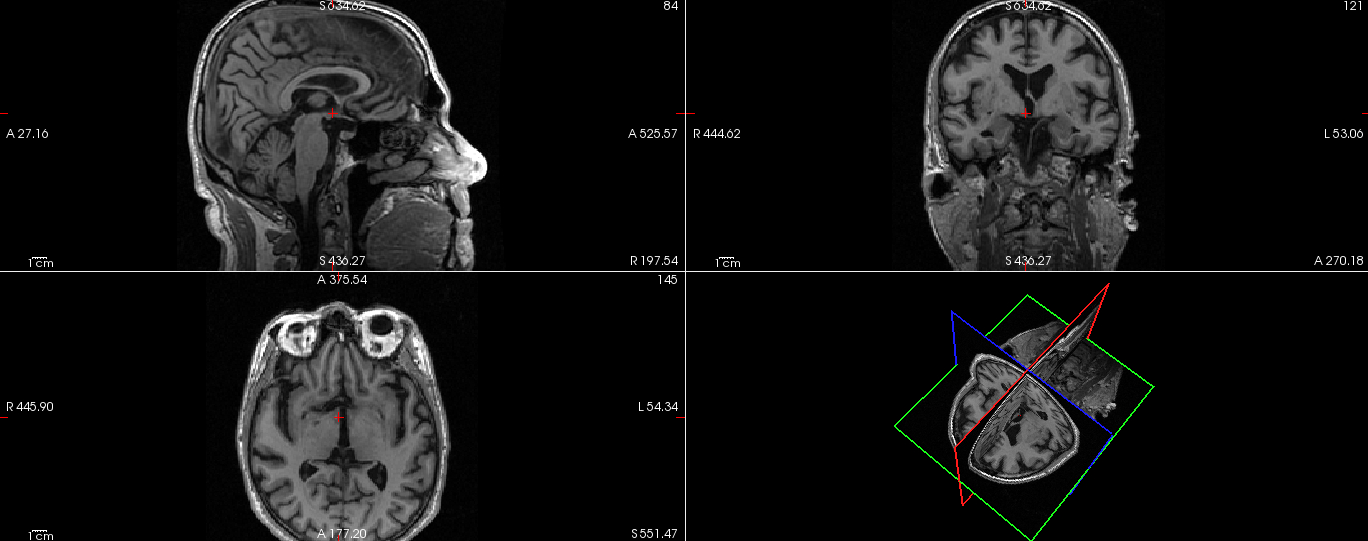
\includegraphics[width=0.95\linewidth]{mymans2}
	\caption{An example of the original image file: \texttt{001.mgz} from subject 002\_S\_0295}
	\label{fig:screenshot001}
\end{figure}


%\begin{figure}
%	\centering
%	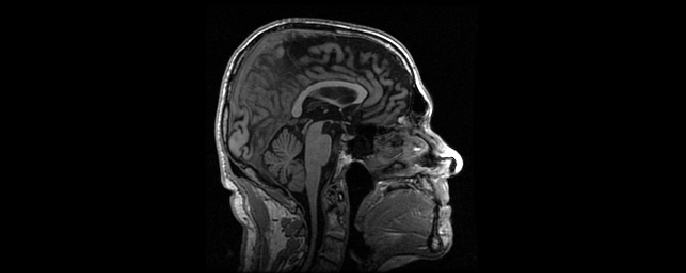
\includegraphics[width=0.7\linewidth]{imgs/mymans_orig_oskar}
%	\caption{}
%	\label{fig:mymansorigoskar}
%\end{figure}


%\begin{table}[H]\label{variable}
%	\centering
%	\begin{tabular}{l l l}
%		\toprule
%		\textbf{Variable} & \textbf{Description} & \textbf{Type} \\ \midrule
%		age & The age of the offenders & Continuous ratio \\
%		priors\_count & The number of previous offences & Discrete interval \\
%		juv\_fel\_count & The number of previous juvenile felonies & Discrete interval \\
%		juv\_misd\_count & The number of previous juvenile misdemeanor & Discrete interval \\
%		c\_charge\_degree & The severity of the offence & Discrete nominal \\
%		race & The race of the offender & Discrete nominal \\
%		age\_cat & The age category of the offender & Discrete nominal \\
%		sex & The sex of the offender & Discrete nominal \\
%		\hdashline
%		score\_text & The COMPAS prediction of chance of recidivism & Discrete interval \\
%		is\_recid & Whether the offender truly recidivated after two years (0/1) & Discrete nominal \\ \bottomrule
%	\end{tabular}
%\end{table} \noindent



\subsubsection{Data Preprocessing}

% We use skullstripped 
% We use normalized 
% Template mni305.cor (what does cor stand for)
% what is in the talairach file 
% mri_vol2vol (What does it do) 

% Indtilvidere skriver om advanced registration, talairach space, etc. her


\subsubsection{Data Augmentation}
% Hvis vi vælger at bruge augmentation

\subsection{Explanation of Data Variables}
%subj_id, age, etc. etc. - dette skal findes et sted på server eller ADNI hjemmeside 

\subsection{Visualization of Data}
% Slices of img, preview 

\subsection{Ethicality of Data}
% Quick rant about GDPR



\section{Methods}
% Short description of all methods
\subsection{Neural Network for Alzheimer's Disease Classification}
In the original Alzheimer's disease classification paper by Camilla, a neural network was used to determine whether each patient had AD. Since this model was full of bias when used on the original data, we used this same model to compare and contrast if the below methods succeeded in removing the most prominent biases from the model. The model was implemented as a PyTorch neural network with 12 convolution layers using ReLU as activation function between each layer. This was followed by a fully connected layer with sigmoid activation to output the probability of each class (sick or healthy). A much more detailed breakthrough of the general project and architecture of the neural network can be seen in \cite{CamillaKandidat}.

\subsection{Generative Adversarial Network}
Since the meat and potatoes of this project is the cycleGAN, the methods and mathematical understanding behind Generative Adversarial Networks (GANs) will only be briefly explored in this section. A GAN was implemented on the MNIST dataset as a preliminary trail to help understand the basics. This implementation can be seen \href{https://github.com/oskarwiese/AlzPred/blob/main/preliminary/GAN_MNIST.ipynb}{here}. This implementation as well as this section will hopefully help to give the proper insight into the reasoning behind cycleGANs later in this section.

In general, GANs can be seen as two different complex neural networks competing for the best accuracy during  the process of generating a class of pictures. In other words, the networks are adversaries in generating or classifying images, from which the source of the name becomes clear. One of the networks will be focusing on generating a fake version of images seen in a training folder, called the \textit{generator}, and the other will be trying to distinguish between real and fake images, called the \textit{discriminator}. This competition between networks leads to results much better than ever seen in ML and AI image generation, thus making a good foundation for the generation of 1.5T fMRI images from 3T. The two networds are covered in depth in the below subsections.
\begin{figure}[H]
	\centering
	\includegraphics[width=0.7\linewidth]{"imgs/GAN architecture"}
	\caption{The GAN architecture. The generator decodes the random noise from the latent space into a fake image. This fake imgae as well as an image from the training set is fed into the Discriminator, which encodes the data into a binary prediction of whether the image is real or fake.}
	\label{fig:gan-architecture}
\end{figure}


\subsubsection{Generator}


\subsubsection{Discriminator}


\subsubsection{Loss}


\subsection{CycleGAN}
% Vigtigt at komme ind på original paper

% F: X -> Y samt G: Y -> X

\subsubsection{General Model Architecture}
% Visualizer library (måske)


\subsubsection{Discriminator in a cycleGAN}

\subsubsection{Generator in a cycleGAN}

\subsubsection{Loss, optimizer, cross Entropy, Etc.}

\subsubsection{Classifier}

\subsection{Reproducibility}\label{repro}


\section{Results}




\section{Discussion}

\subsection{Would the Model be Efficacious in Practice?}

\subsection{Standardization of Measuring Equipment (3T/1.5T)}

\subsection{Improvements for Future Papers}

\subsection{Dealing With GDPR in Personal Data}

\subsection{Safe AI}



\section{Conclusion}



\newpage
\section{Appendix}

\subsection{Pseudo Code}

\subsection{Batch script}





\newpage
\begin{thebibliography}{9} 
	
%	\bibitem{tv2} K. Andreasen "Flere end 15.000 deltog i dansk Black Lives Matter-demonstration", 2020 Tv2 Lorry, at \url{https://www.tv2lorry.dk/koebenhavn/15000-mennesker-samles-til-dansk-demonstration-mod-racisme-mod-racisme}, visited 19-06-2020
	
%	\bibitem{cnn1}  M. Macaya et al. "June 17 Black Lives Matter protests news", 2020 CNN, at \url{https://edition.cnn.com/us/live-news/black-lives-matter-protests-06-17-2020/index.html}, visited at 19-06-2020
	
%	\bibitem{cnn2} M. Macaya et al. "June 18 Black Lives Matter protests news", 2020 CNN, at \url{https://edition.cnn.com/us/live-news/black-lives-matter-protests-06-18-2020/index.html}, visited 19-06-2020
		
		
		\bibitem{first} Zhu, Jun-Yan, et al. "Unpaired image-to-image translation using cycle-consistent adversarial networks." Proceedings of the IEEE international conference on computer vision. 2017.
		
		\bibitem{second} Burns, Jeffrey M., et al. "Reduced lean mass in early Alzheimer disease and its association with brain atrophy." Archives of neurology 67.4 (2010): 428-433.
		
		\bibitem{CamillaKandidat} Pedersen, Camilla Kergel "Demographic bias in public neuroimaging databases, and its effect on AI systems for computer-aided diagnosis." University of Copenhagen Faculty of Science. 2021.
		
		\bibitem{adni}  Alzheimer’s
		Disease Neuroimaging Initiative homepage: \url{http://adni.loni.usc.edu/}, last visited at 
		28 Nov. 2021
		
		\bibitem{adni1} Alzheimer’s
		Disease Neuroimaging Initiative about ADNI1 \url{http://adni.loni.usc.edu/about/adni1/}, last visited at 28 Nov. 2021
		
	\end{thebibliography}
	
	
	\newpage
	\bibliographystyle{IEEEbib}
	\bibliography{refs}
\end{document}
